
\begin{figure}[ht]
  \centering
  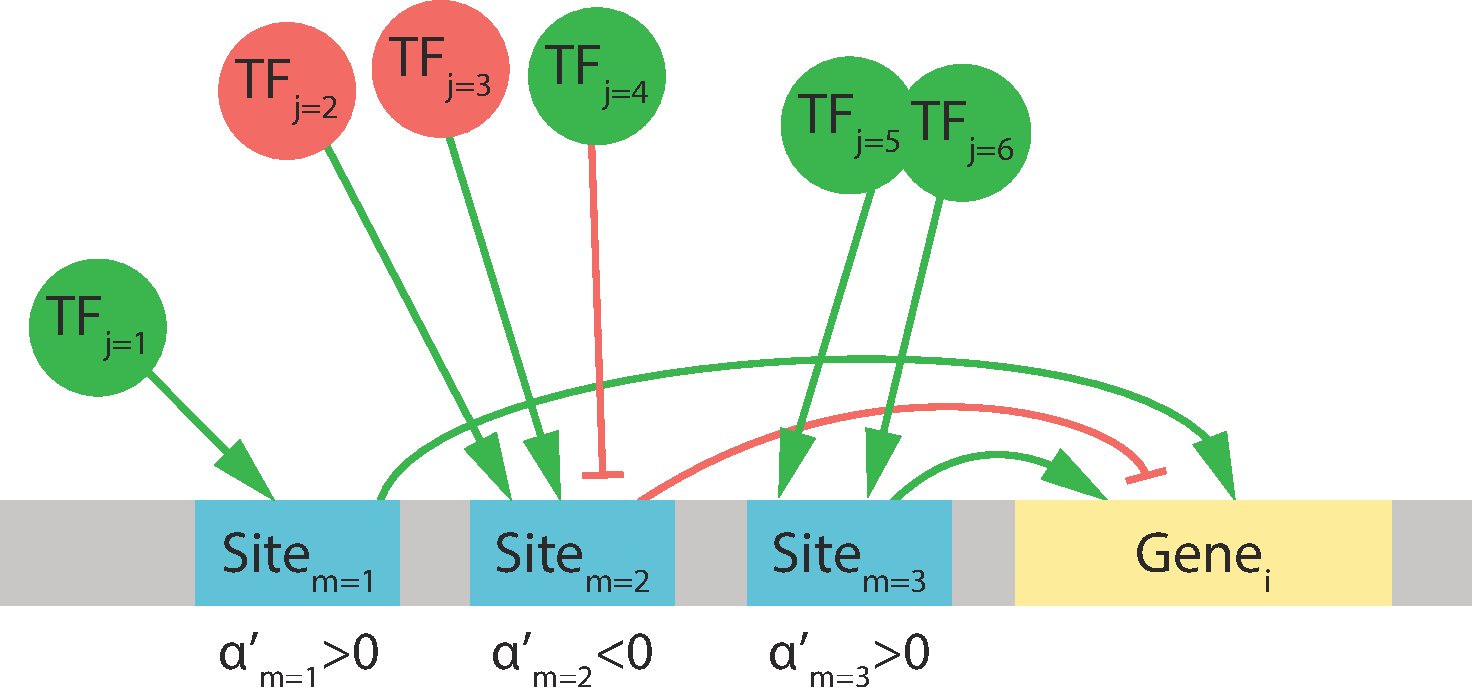
\includegraphics[width=\textwidth]{theory/fig/GeneWeaverRegulation.pdf}
   \caption{\textbf{Example of transcriptional regulation in simulation.}
    A gene regulated by $N=3$ regulatory modules, where module 1 is regulated by a single activator TF, module 2 is bound by a complex of two TFs, which both have to be present for activation of the module, and activating and repressing TFs compete to bind the third module. \textcolor{OliveGreen}{Green}: activation, \textcolor{red}{red}: repression.} 
  \label{fig:gnw_regulation}
\end{figure}


